\title{%
  \Huge{\textbf{Interactive Tool for Teaching Hindley-Milner Type Inference through Visualisation}}
  \\
  \Large{Final report\\~\\~\textbf{Adam Jones}\\~Department of Computer Science\\~University of Warwick}
}

\documentclass[a4paper,fleqn,12pt]{article}

\usepackage[]{geometry}
\usepackage[utf8]{inputenc}
\usepackage[UKenglish]{babel}
\usepackage[UKenglish]{isodate}
\usepackage{amsmath}
\usepackage{amsfonts}
\usepackage{amssymb}
\usepackage{amsthm}
\usepackage{graphicx}
\usepackage{chngpage}
\usepackage{calc}
\PassOptionsToPackage{hyphens}{url}
\usepackage{hyperref}
\usepackage[nameinlink]{cleveref}
\usepackage{fancyhdr}
\usepackage{titletoc}
\usepackage[explicit]{titlesec}
\usepackage{natbib}
\usepackage[dvipsnames]{xcolor}
\usepackage[sc]{mathpazo}
\linespread{1.05} 
\usepackage[T1]{fontenc}
\usepackage{minted}
\usepackage{ragged2e}
\usepackage{adjustbox}
\definecolor{cs310lightgrey}{rgb}{0.95,0.95,0.95}
\usepackage[backgroundcolor=cs310lightgrey,hidealllines=true]{mdframed}

\hypersetup{
	colorlinks=true,
	linkcolor=black,
	urlcolor=black,
	citecolor=black
}

\BeforeBeginEnvironment{minted}{\begin{mdframed}}
\AfterEndEnvironment{minted}{\end{mdframed}}

\let\parencite\citep

\setlength{\parindent}{0mm}
\setlength{\parskip}{\medskipamount}
\renewcommand\baselinestretch{1.2}

\cleanlookdateon

\pagestyle{plain}
\renewcommand{\headrulewidth}{0.0pt}

\makeatletter
\fancypagestyle{plain}{
	\fancyhf{}
	\fancyhead[RE,RO]{\thepage}
	\fancyhead[LE,LO]{\textit{Interactive Tool for Teaching HM Type Inference through Visualisation}}
}
\makeatother

\begin{document}

\makeatletter
\begin{titlepage}

\LARGE \@title \\
\Large \\[1.5cm]

\vfill 

\begin{adjustwidth}{-\oddsidemargin-1in}{-\rightmargin}
  \centering
  
\includegraphics[width=\paperwidth]{line.png}
\end{adjustwidth}

\vspace*{-3.5cm}

\end{titlepage}
\makeatother

\pagestyle{plain}

\begin{figure}[h!]
  \centering
  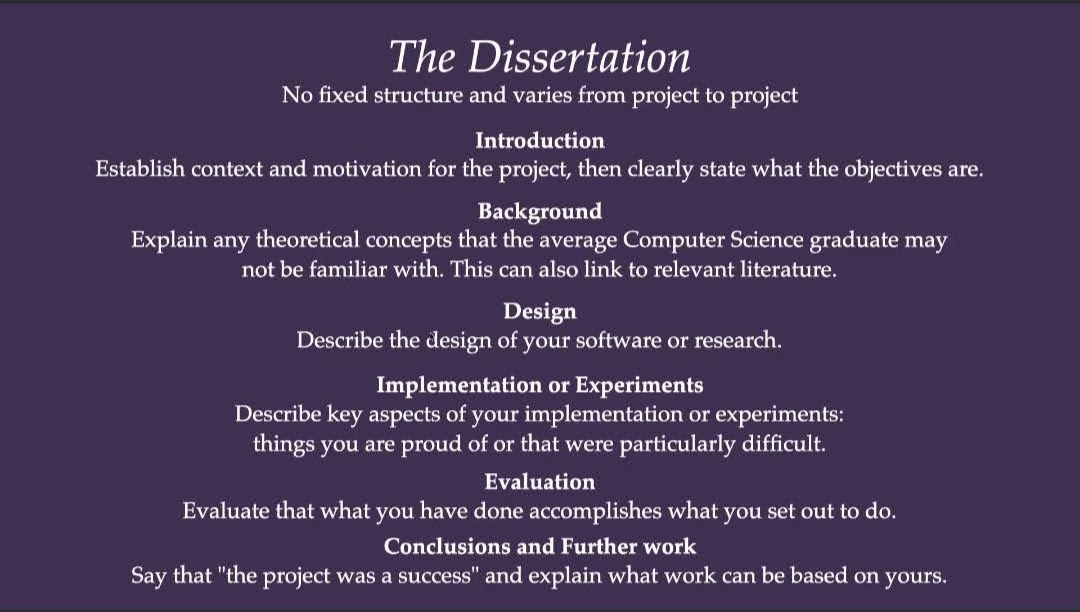
\includegraphics[width=1.000\linewidth]{images/image4.jpg}
  \caption{Screenshot from mbg presentation on structure}
\end{figure}

TODO: Abstract, keyword list?

\section{Introduction}\label{id:h.6k9gcmunzldy}

Types in programming languages specify what values an element of a computer program may take. These include primitive data types such as integers, booleans and characters and more complex types such as class or function types.

Programs can be checked for type-errors, either at runtime (dynamic type checking) or compile time (static type checking). Type checking identifies issues with types and throws either runtime or compile errors when an invalid operation has occurred, for example applying a function accepting an integer to a boolean. This is primarily used to catch bugs in program code, preventing unexpected behaviour.

Static type checking can prevent type errors from occurring at runtime. This is particularly useful when code paths may not be well-tested or frequently used, as runtime checks only surface type errors when the problematic code is executed. Additionally, static type checking allows for better tooling that improves developer productivity. For example, IDEs may use type information to suggest and perform automated refactorings \citep{ref1}, automatically generate documentation \citep{ref2} and autocomplete statements \citep{ref3}.

Some languages allow the programmer to override static type checking results, in cases where they know more than the type checker about a particular part of a program. For example Java allows casting an object to its subclass and TypeScript has its `as` type assertion operator and `any` and `unknown` types. These can be used sparingly (and often in combination with `instanceof` and `typeof` operators respectively) by programmers as an escape hatch to work around the type checker’s limitations. In these situations, runtime checks are often performed to maintain type safety, for example with Java throwing a `ClassCastException`.

```java

// MySubclass extends MyClass

// MyOtherSubclass extends MyClass

MyClass c1 = new MySubclass();

MySubclass s1 = (MySubclass) c1; // okay

MyClass c2 = new MyOtherSubclass();

MySubclass s2 = (MySubclass) c2; // throws ClassCastException at runtime

```

Casting an object to its subclass in Java

```typescript

const a = Math.random() < 0.5 ? 'cs310' : 310; // has type "cs310" | 310

const b = a + a; // throws a type error, but b could have type "cs310cs310" | 620

const c = a == 'cs141' ? a + a : a + a; // okay, has type number | string

const d = a as any + a; // okay, has type any

const e = a as any + a as 'cs310cs310' | 620 // okay, has type "cs310cs310" | 620

// @ts-ignore

const f: 'cs310cs310' | 620 = a + a; // okay, has type "cs310cs310" | 620

```

Some type-safe code is rejected by the TypeScript type checker, but there are many possible workarounds

As static type checking is performed at compile time, generally the code must have enough information to deduce its types without runtime arguments. This may be in the form of type annotations or typed variable and function declarations. However, specifying types manually can be time-consuming and potentially difficult.

A type inference algorithm for a particular programming language’s type system can determine types automatically, which improves productivity by allowing programmers to get the best of types without having to explicitly specify them. Because of this, type inference is used in many popular programming languages with expressive type systems including Haskell, Rust and TypeScript.

An understanding of type inference would help computer scientists write cleaner code and debug type errors. However, few universities have core modules on type systems (although they may be touched on in programming curriculums) and there are limited easy-to-understand teaching resources on type inference. Therefore, many computer science graduates will be missing a useful understanding of how type inference actually works.

\subsection{Related work}\label{id:h.2mwaav7jkal4}

TypeTool by~\cite{ref4} was a tool that visualised type inference through a web application, and was found to be beneficial for teaching purposes. Users entered an expression in a custom expression language, submitted a request to a server and were redirected to a page displaying an initial syntax tree, a final syntax tree and an overall substitution.

{\centering \begin{figure}[h!]
  \centering
  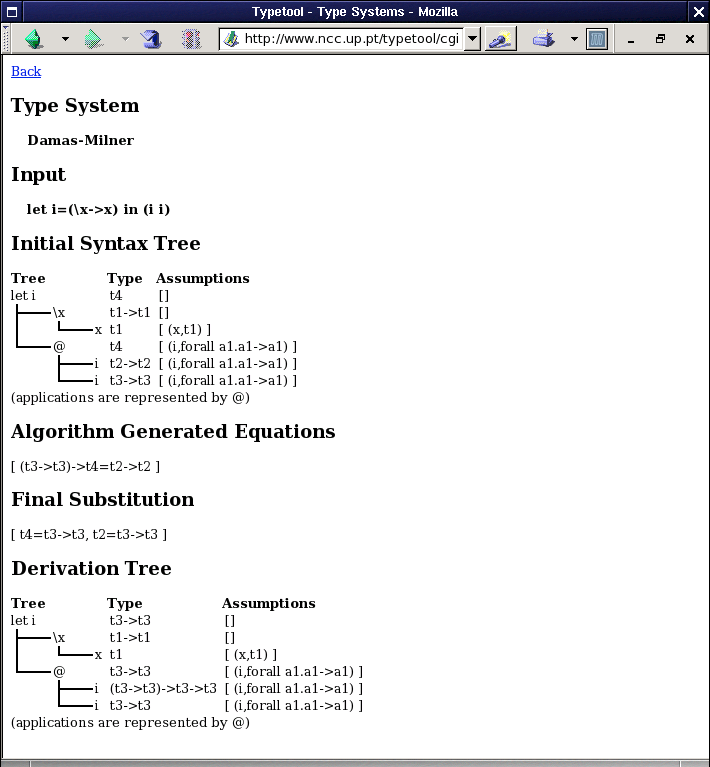
\includegraphics[width=0.770\linewidth]{images/image2.png}
  \caption{Screenshot of results from TypeTool, taken from their paper}
\end{figure} \par}

By allowing users to enter their own expressions, students can explore how the systems work in different cases to gain an intuitive understanding of the concepts. This interactive approach improves understanding as users can easily try testing their own assumptions or examine edge cases they are unsure of.

Unfortunately, the tool is now inaccessible as the server hosting the application is no longer running and the source code has not been published. Additionally, as the parsing and type inference was done server-side there was a delay between the user entering an expression and seeing the result. While short, a delay reduces the ease-of-use and may discourage users from trying many different expressions. Both delayed feedback and the lack of step-by-step explanations reduce learning quality \citep{ref5}, particularly in the area of rule learning;~\cite{ref6} showed that immediate explanatory feedback is most effective at learning how to apply rules in computer programming. It is unclear what the output of the tool with incorrectly-typed expressions is.

Despite these shortcomings, TypeTool’s authors found in teaching the University of Porto’s functional programming course that the tool was “especially useful for students, because it helps to understand the type systems of the most common typed functional languages” and that “[presenting] the basis of type inference technology [...] significantly improved the way students deal with type errors because they understand the type system.”

\cite{ref7} developed a visual functional programming system which visualises types during function application for a subset of Standard ML, used to teach first year undergraduate students. However, this did not explicitly show the type inference process and as a desktop application rather than web app it is less accessible to lecturers and students. It also didn’t support key functional language constructs such as function declarations and let bindings, and required significant explanation before using the tool to understand its output.

{\centering \begin{figure}[h!]
  \centering
  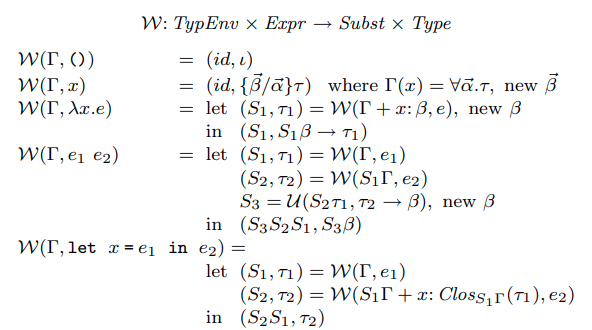
\includegraphics[width=0.797\linewidth]{images/image1.png}
  \caption{Screenshot of Yung and Michaelson's tool, taken from their paper}
\end{figure} \par}

NiMo \citep{ref8} is a graphical programming language related to functional data processing which allows users to reason about the flow of data through a program. The types of data and processes can be inspected in NiMoToons, and type inference is performed over the network of components. However, larger expressions can become complicated and be difficult to interpret. While NiMo performs type inference internally it is not a key focus to the end-user, and as such does not explain its steps. Additionally, it is harder to relate back to more commonly used, textual functional languages like Haskell.

{\centering \begin{figure}[h!]
  \centering
  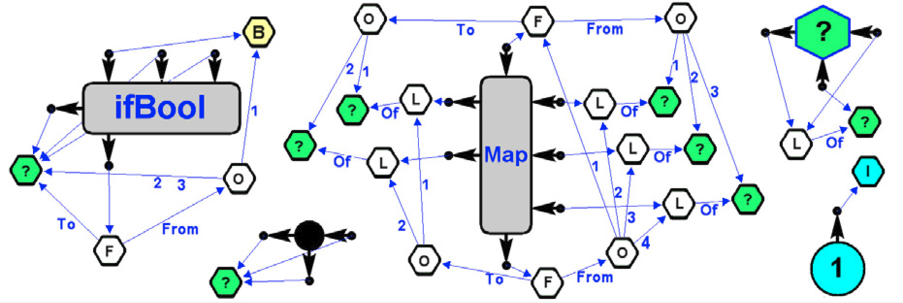
\includegraphics[width=0.960\linewidth]{images/image3.png}
  \caption{A diagram showing the types of some variables in NiMo, taken from their paper}
\end{figure} \par}

\cite{ref9} implemented a successful teaching tool, named TILC, for visualising lambda-calculus parse trees in order to help with teaching lambda-calculus to undergraduate students. They noted that to develop an intuitive understanding, students would benefit from  experimenting with lambda-calculus and that “a tool that deals with all these aspects in a friendly and graphical manner incentivises [experimentation]”. TILC was successful, with the module organisers of ‘programming paradigms’ at the Universitat de Girona having a “good experience of using this tool in the course lectures and as a downloadable tool for students”. The authors suggested extending TILC to show types and type inference would have pedagogical value.

To summarise, types (such as integers, booleans and functions) aid the construction of correct programs. Type checking can detect errors in programs, called \textit{static} when run at compilation time and \textit{dynamic} if run as the program executes. Type inference is a method often used alongside static type checking to determine types in a program, an understanding of which could benefit computer scientists in writing and debugging programs. Some solutions exist which give students a better idea about types, however they either have significant limitations or do not explicitly cover type inference.

\subsection{Objectives}\label{id:h.o72kh3tf0r5l}

The ultimate goal of the project is to improve undergraduate students’ knowledge and understanding of how type inference works.

To achieve this, this project will develop a teaching resource that explains how type inference algorithms work for functional languages. An interactive web application will allow students to enter expressions and view the results of a type inference algorithm, along with the steps taken to get to that result. This would be particularly useful in the context of modules teaching functional languages such as Haskell which perform similar type inference.

\section{Background}\label{id:h.ebjyqi73zdyo}

\subsection{$\lambda$-calculus}\label{id:h.odw4vku9eizz}

A $\lambda$-calculus is a representation of computation. Generally these have at least 3 key constructs:

\begin{itemize}
  \item `var`: Variables
  \item `abs`: Function abstraction, defining anonymous functions
  \item `app`: Function application, applying subexpressions to each other
\end{itemize}

For example, consider the expression:

```

($\lambda$x. x) y

```

It has variables `x` and `y`. Variables may be bound or free (unbound). Here `x` is bound as it is a parameter in the function abstraction, and `y` is free as there is nothing which binds it. This can be thought of in a similar way to how variables in most imperative programming languages have a scope where they are defined or undefined.

The function abstraction mentioned is the `$\lambda$x. x` part. This defines an anonymous function which given an argument (before the full stop) `x` simply returns (after the full stop) `x`, i.e. the identity function. A function to add three to an input might be written `$\lambda$x. x + 3` (although many of the most fundamental $\lambda$-calculi do not have such explicit notions of addition or numbers).

Functions may be returned by other functions, which enables functions to have the appearance of taking multiple arguments. For example `$\lambda$x. ($\lambda$y. x)` can be viewed as a function which takes two arguments and then returns the first one. Here explicit brackets have been given for clarity, but they aren’t necessary. Additionally, sometimes multiple arguments like this are written together, so `$\lambda$x. ($\lambda$y. x)`, `$\lambda$x. $\lambda$y. x` and `$\lambda$xy. x` all mean the same thing.

Finally, the function application is actually applying the function `$\lambda$x. x` to the argument `y`. In $\lambda$-calculus evaluation is performed via $\beta$-reductions. In our example this could be done by substituting the argument `y` for parameter `x` in the body of the function `x`, resulting in `y`.

This expression’s construction can be represented as an abstract syntax tree:

TODO: tree diagram of the expression

In addition to these three constructs, a `let` construct is added to some calculi to allow binding a value to a variable in an expression. For example `let x = 3 in x * x` binds `x` to the value `3` in `x * x`. A `lit` construct may be added to represent literal constants, such as numbers or booleans like `3` and `True`.

$\lambda$-calculi have been extensively studied, often using formal inductive definitions. For example, the inductive definition for the set of free variables in an expression based on the constructors introduced so far is:

\begin{itemize}
  \item `var`: \$FV(x) = \{ x \}\$
  \item `abs`: \$FV($\lambda$x. E) = FV(E) - \{ x \}\$
  \item `app`: \$FV(E\_1 E\_2) = FV(E\_1) $\cup$ FV(E\_2)\$
  \item `let`: \$FV(let x = E\_1 in E\_2) = FV(E\_2) - \{ x \}\$
  \item `lit`: \$FV(c) = $\varnothing$\$
\end{itemize}

where E is any expression. Given these rules the set of free variables for any combination of these constructs can be determined. This can be demonstrated for our example expression `($\lambda$x. x) y`, which is shown in a tree structure below. More generally this is an example of how an inductive definition can tell us something about the entire program which is how some type inference algorithms can be viewed.

TODO: tree diagram of the expression with the sets of free variables at each node.

Most real-world environments define a context which binds some variables by default to in-built values. For example Haskell’s GHC primitives and Prelude includes basic variables like `[]` (the empty list) and `not` (a function which inverts booleans). These can be considered bound at the top level and removed from the set of free variables there.

\subsection{The simply typed $\lambda$-calculus}\label{id:h.w7vj0r89b86n}

Typed $\lambda$-calculi extend the system with the concept of types.

The simply typed $\lambda$-calculus is one of the simplest typed $\lambda$-calculi, and introduced by~\cite{ref10} is often viewed as the canonical typed $\lambda$-calculus. It has the `var`, `abs`, `app` and `lit` constructs. Types in this system are either base types (often in the literature Greek letters $\alpha$, $\beta$, $\gamma$ are used, but these can be thought of similar to numbers, booleans, characters etc.) or functions between other types (such as `Int -> Bool`, or `Int -> (Bool -> Bool)`). The syntax is modified to add type annotations to `var`, `abs` and `lit` constructs, for example `($\lambda$x: Int. odd\textsuperscript{Int -> Bool} x\textsuperscript{Int}) 3\textsuperscript{Int}` (although often for simplicity the types of `var` and `lit` subexpressions, those in superscript, are left out).

\subsection{Hindley-Milner type system}\label{id:h.gsouq2axz3k}

Hindley-Milner (HM) is a typed $\lambda$-calculus which allows for the types of programs to be inferred and no type annotations are required \citep{ref11,ref12}. It extends the simply typed $\lambda$-calculus by adding `let` bindings and a richer type system that includes \textit{type functions} and \textit{polymorphism}.

Like expressions, types can be considered to be built from `var` variables and `app` function applications. Type variables are either base types like `Bool` and `Int` or type functions. Type functions can be applied, taking types as parameters to construct composite types. For a type to be valid all functions must be fully applied, unlike expressions where the final expression may be a function.  As with expressions, we can again assume a global context that binds the basics like `Bool`, `Int` and `->`. In Hindley’s original paper only `->` was considered as a type function, however here we explore several type functions that have been found useful in practice.

The type function we’ve already been using is the function type function, `->`. It takes two types as arguments and represents a function from the first type to the second. A function from `Int` to `Bool` is represented by `(->) Bool Int` in prefix notation, although would more commonly be written infix as `Bool -> Int`. The function type function (`->`) should not be confused with the function type: an expression representing a function has a function type, and that function type is the function type function applied to arguments. For example `$\lambda$x. x + 3` has a function type `Int -> Int`, which is the function type function `->` applied to arguments `Int` and `Int`.

The list type function is also very common, which given one type argument represents a list of those types. A list of booleans might be written `List Bool` or `[] Bool` in prefix notation, although often the list type is represented by wrapping the type argument in square brackets instead like `[Bool]`.

`Maybe` is another type function commonly used in functional languages like Haskell. A `Maybe` represents the optional presence of something, similar to Java’s `Optional` and C++’s `std::optional`. Applied to a boolean type this may be written `Maybe Bool`, representing a wrapper around nothing or a boolean. In Java this would be represented with a generic as `Optional<Boolean>` and in C++ `std::optional<bool>`.

Other common type functions include `Either` and tuples. `Either` takes two type arguments and represents a wrapper around either one of the types, e.g. an either for a boolean or integer is written `Either Bool Int`. Tuple constructors are a set of type functions representing a cross product of their type arguments, named `,`, `,,`, `,,,` and so on for different element lengths. A 3-tuple holding a boolean, integer and integer can technically be written in prefix notation as `(,,) Bool Int Int` but instead generally tuples borrow mathematical syntax with parentheses and commas like `(Bool, Int, Int)`.

The set of types made from `var` and `app` are known as monotypes. For example, `Bool`, `Int`, `Bool -> Int`, and `Bool -> [(Bool, Int -> Maybe Bool)]` are all monotypes.

Adding zero or more for-all qualified type variables to monotypes forms polytypes (called principal type schemes by Hindley and polymorphic types by Milner). This can be thought of as the `abs` equivalent for types, written as `$\forall$x. $\rho$` where `$\rho$` is a polytype. This definition makes monotypes a special case of polytypes: monotypes are polytypes with zero for-all qualified type variables.

Polytypes allow for parametric polymorphism, where a type may be parameterized by a for-all bound quantifier. This allows functions to accept different types as long as they meet certain constraints. For example the `length` function is polymorphic: it has the polytype `$\forall$x. [x] -> Int`, which accepts a list of any type and returns its length as an integer. It accepts different types such as `[Bool]` and `[Int -> Bool]` as both of these meet the constraint of being a list.

Correctly inferring polymorphic types can be difficult, and in fact~\cite{ref13} proved that doing so for System F, a type system similar to Hindley-Milner with fewer typing rule constraints, is undecidable. To avoid this, HM chooses not always generalise to the most generic type in function abstraction [TODO: why not treat them like let bindings and institate them with a for-all qualifier?]. As a workaround, it adds `let` bindings which allows for binding variables to values with polymorphic types explicitly by generalising the type of the bound variable.

This is the difference between:

\begin{itemize}
  \item `let i = (\textbackslash x -> x) in (i 3, i True)` type-checks, as i is generalised to the polytype `$\forall$a. a -> a` so can be applied to both an `Int` and `Bool`
  \item `(\textbackslash i -> (i 3, i True)) (\textbackslash x -> x)` does not type-check as i has the monotype `a -> a`, and `a` must take only one type in both tuple parts.
\end{itemize}

Hindley-Milner is the basis for the type system of Standard ML \citep{ref14} (which OCaml and F\# are related to) and was the basis of the type system in Haskell \citep{ref15}.

\underline{\href{http://smallcultfollowing.com/babysteps/blog/2017/03/25/unification-in-chalk-part-1/}{http://smallcultfollowing.com/babysteps/blog/2017/03/25/unification-in-chalk-part-1/}}

\underline{\href{https://perplexinglyemma.blogspot.com/2017/06/language-servers-and-ides.html}{https://perplexinglyemma.blogspot.com/2017/06/language-servers-and-ides.html}}

\underline{\href{https://www.reddit.com/r/rust/comments/6fs5q9/language\_servers\_and\_ides/dikywtc/}{https://www.reddit.com/r/rust/comments/6fs5q9/language\_servers\_and\_ides/dikywtc/}}

Looks maybe useful - talks about unification and type inference, although from a fairly Rust-y perspective (and I’ve never touched Rust before…)

\underline{\href{https://apple-swift.readthedocs.io/en/latest/TypeChecker.html}{https://apple-swift.readthedocs.io/en/latest/TypeChecker.html}}

“Swift implements bi-directional type inference using a constraint-based type checker that is reminiscent of the classical Hindley-Milner type inference algorithm.” ... “The Swift language contains a number of features not part of the Hindley-Milner type system, including constrained polymorphic types and function overloading”.

Haskell has since been extended with type-class constraints \citep{ref16}, functional dependencies \citep{ref17}, and generalised algebraic data types (GADTs) \citep{ref18}. Haskell’s inference engine was moved onto a new engine, OutsideIn(X), when GHC 7.2 was released November 2011 after~\cite{ref19} proposed a solution to the issues with Hindley-Milner’s poor performance on large programs and difficulty inferring expressions without principal types that arise with type-class constraints and GADTs. In doing this, Haskell stopped automatically generalising variables bound by `let` expressions after~\cite{ref20} argued that generalising `let` bindings is complex in type inference engines other than HM and the feature was rarely used in practice, with the change only affecting 0.13\% lines of the GHC core libraries.

For the purposes of the teaching tool HM gives a good representation of how type inference works to students while not being too complex to understand, and is related to how languages commonly used in practice perform type inference.

\subsection{Hindley-Milner type inference}\label{id:h.admfqf7bhkct}

Various algorithms are available to infer types in Hindley-Milner such as Algorithm W by~\cite{ref21} and Algorithm M by~\cite{ref22}. Algorithm W takes a bottom-up approach, attempting to unify the types of subexpressions up the abstract syntax tree, while Algorithm M takes a top-down approach, unifying types down the tree.

Both algorithms sometimes produce poor type error messages; Algorithm W often detects errors late, highlighting too large of a subexpression to be useful and Algorithm M often detects too specific of a term without context as to what original definition it violates. Because of this, hybrid or constraint-based algorithms along with heuristics are often used in practice to provide more informative error messages. Additionally, despite not being required, explicit type annotations are often used to help identify errors earlier at locations which are easier to interpret \citep{ref23}. Type annotations can also act as documentation to future programmers using or working on the code, as sometimes the most general type as worked out by a type inference algorithm may not convey the intent of the programmer most clearly.

TODO: substitutions, contexts, unification

TODO: typing rules

TODO: algorithm W and M definitions?

\underline{\href{https://aaltodoc.aalto.fi/bitstream/handle/123456789/42719/master\_Mikkonen\_Juuso\_2020.pdf}{https://aaltodoc.aalto.fi/bitstream/handle/123456789/42719/master\_Mikkonen\_Juuso\_2020.pdf}}

Talks about statically typed languages in JavaScript-land. Mentions things like TypeScript don’t use HM because JS has a lot of structural typing (i.e. if objects have the right properties it’s fine to call methods that depend on that interface) and subtyping.

\underline{\href{https://research.cs.queensu.ca/home/jana/papers/bidir/Dunfield13\_bidir.pdf}{https://research.cs.queensu.ca/home/jana/papers/bidir/Dunfield13\_bidir.pdf}}

I seem to have come across this paper quite a few times. I still don’t really understand it, but it seems important.

\underline{\href{https://www.sigmacomputing.com/blog/writing-a-parser-combinator-from-scratch-in-typescript/}{https://www.sigmacomputing.com/blog/writing-a-parser-combinator-from-scratch-in-typescript/}}

Parser in TypeScript

\underline{\href{https://tomassetti.me/parsing-in-javascript/}{https://tomassetti.me/parsing-in-javascript/}}

Parsing in JavaScript - lots of library recommendations (see Parjs and Jison)

\underline{\href{http://reasonableapproximation.net/2019/05/05/hindley-milner.html}{http://reasonableapproximation.net/2019/05/05/hindley-milner.html}}

A reckless introduction to Hindley-Milner type inference

\underline{\href{https://en.wikipedia.org/wiki/Types\_and\_Programming\_Languages}{https://en.wikipedia.org/wiki/Types\_and\_Programming\_Languages}}

Book recommended by mbg

\underline{\href{https://homepages.inf.ed.ac.uk/wadler/papers/papers-we-love/milner-type-polymorphism.pdf}{https://homepages.inf.ed.ac.uk/wadler/papers/papers-we-love/milner-type-polymorphism.pdf}}

Original algorithm W paper

\underline{\href{https://www.dcs.warwick.ac.uk/michael\_gale/publications/wsiw.pdf}{https://www.dcs.warwick.ac.uk/michael\_gale/publications/wsiw.pdf}}

Michael’s what should I wear paper

\underline{\href{http://citeseerx.ist.psu.edu/viewdoc/download?doi=10.1.1.65.7733\&rep=rep1\&type=pdf}{http://citeseerx.ist.psu.edu/viewdoc/download?doi=10.1.1.65.7733\&rep=rep1\&type=pdf}}

\underline{\href{https://gist.github.com/paf31/a49a54d7ea5ede43422f}{https://gist.github.com/paf31/a49a54d7ea5ede43422f}}

Implementing algorithm W in Haskell

\underline{\href{https://codeburst.io/https-chidume-nnamdi-com-npm-module-in-typescript-12b3b22f0724}{https://codeburst.io/https-chidume-nnamdi-com-npm-module-in-typescript-12b3b22f0724}}

Typescript library template

\underline{\href{https://www.researchgate.net/profile/Jurriaan\_Hage/publication/221241370\_Scripting\_the\_Type\_Inference\_Process/links/02e7e51a37f9233c65000000.pdf}{https://www.researchgate.net/profile/Jurriaan\_Hage/publication/221241370\_Scripting\_the\_Type\_Inference\_Process/links/02e7e51a37f9233c65000000.pdf}}

Improving type error messages

\underline{\href{https://dspace.library.uu.nl/bitstream/handle/1874/7297/full.pdf?sequence=8}{https://dspace.library.uu.nl/bitstream/handle/1874/7297/full.pdf?sequence=8}}

Top quality type error messages

\underline{\href{https://manu.sridharan.net/files/mycroft-preprint.pdf}{https://manu.sridharan.net/files/mycroft-preprint.pdf}}

A Practical Framework for Type Inference Error Explanation

\underline{\href{https://theory.stanford.edu/\textasciitilde aiken/publications/trs/FLProject.pdf}{https://theory.stanford.edu/\textasciitilde aiken/publications/trs/FLProject.pdf}}

Designing a FP language

\underline{\href{http://citeseerx.ist.psu.edu/viewdoc/download?doi=10.1.1.110.5050\&rep=rep1\&type=pdf}{http://citeseerx.ist.psu.edu/viewdoc/download?doi=10.1.1.110.5050\&rep=rep1\&type=pdf}}

PhD thesis which talks about hindley milner and type inference a lot

\underline{\href{http://www.reflection.uniovi.es/ortin/publications/visual-2014.pdf}{http://www.reflection.uniovi.es/ortin/publications/visual-2014.pdf}}

Hybrid dynamically and statically typed languages

\underline{\href{http://lucacardelli.name/papers/typesystems.pdf}{http://lucacardelli.name/papers/typesystems.pdf}}

Paper that introduces the basics of type systems and types n’ stuff

\underline{\href{https://citeseerx.ist.psu.edu/viewdoc/download?doi=10.1.1.5.4267\&rep=rep1\&type=pdf}{https://citeseerx.ist.psu.edu/viewdoc/download?doi=10.1.1.5.4267\&rep=rep1\&type=pdf}}

Algorithm W’, the symmetric unification one

\section{Design}\label{id:h.7ggvdxb04tzm}

???

\section{Implementation}\label{id:h.igepudpadp49}

Developed gdoc2latex

Set up CI system to build latex docs

Tried using Docker to run latex compilation step in GitHub actions, but found it was significantly slower (2 mins vs 45 seconds) than installing texlive-latex-extra and texlive-bibtex-extra on the runner directly.

Implemented algorithm W in a mix of class-based and functions, then reimplemented to be just functions.

Added custom test matcher

How the step logging works

How does the web app work, performance analysis and considerations

Analytics

Adding algorithm M

\section{Evaluation}\label{id:h.e6letww4nhn0}

Maybe also analyse performance?

Compare to existing available libraries?

Test on people?

Look at the analytics?

\section{Conclusions and Further Work}\label{id:h.fc67ipatea73}

\section{Ethics}\label{id:h.i0n8c6hqdr6j}

\section{Acknowledgements}\label{id:h.xqaef57orpsv}

This document was typeset using a derivative of the CS310 starter pack\footnote{\href{https://github.com/mbg/cs310}{https://github.com/mbg/cs310}} by Michael Gale, licensed under CC BY 4.0.

\bibliography{index}

\bibliographystyle{./plainnat}

\end{document}